We use vue.js (TODO citation) as the UI framework for our tool, combined with PrimeVue (TODO citation) as the UI component library and Tailwind CSS (TODO citation) for CSS utility.
A detailed list of all libraries used can be found in the wiki of our GitHub repository (TODO link).
Table~\ref{tab:libraries} shows an overview of the most important libraries used and their purpose.

% todo insert most important libraries used and their purpose
\begin{table*}[!hb] % Use table* for wide tables
    \caption{Libraries used in the implementation of our tool} %keyuri
    \label{tab:libraries}
    \centering
    \begin{tabular}{ll}
        \toprule
        \textbf{Library} & \textbf{Purpose}     \\
        \midrule
        vue.js           & UI framework         \\
        PrimeVue         & UI component library \\
        Tailwind CSS     & CSS utility          \\
        @fortawesome/fontawesome-svg-core & Font Awesome SVG icons. \\
        ajv@8.12.0 & JSON schema validator for Node.js and browsers. \\
        brace@0.11.1 & Browser-based code editor with syntax highlighting and code folding. \\
        primeicons@6.0.1 & It is a popular UI component library for JavaServer Faces (JSF) applications. \\
        \bottomrule
    \end{tabular}
\end{table*}

\subsection{Tool Overview}\label{subsec:tool-overview} %keyuri


The tool provides a solution for managing \cfgfiles{} with three distinct views:
\begin{itemize}
    \item \textbf{File Editor} (Figure~\ref{fig:fileeditor}): For editing \cfgfiles{}, based on the schema provided to the tool.
    \item \textbf{Schema Editor} (Figure~\ref{fig:schemaeditor}): For editing the schema, which is used by the File Editor.
    \item \textbf{Settings} (Figure~\ref{fig:settings}): To configure various tool settings.
\end{itemize}

The user interface of \toolname{} is structured in the following way (see the numbers in red in figure~\ref{fig:fileeditor}):
\begin{enumerate}
    \item Button to switch to another view (e.g., from File Editor to Schema Editor).
    \item Toolbar with various functionality.
    \item Code editor panel.
    \item GUI editor panel.
\end{enumerate}
% While these views may share a similar appearance in the figure, each number assigned to them serves a distinct purpose.
% The first number corresponds to different views, allowing users to switch between the Schema Editor,File Editor and Settings, the second number pertains to the toolbar, functionalities for each view listed following, the third number represents the Code Panel, and the fourth number designates the GUI Panel on the right. We will discuss the unique functions of each of these views in the following sections.

\begin{figure*}
    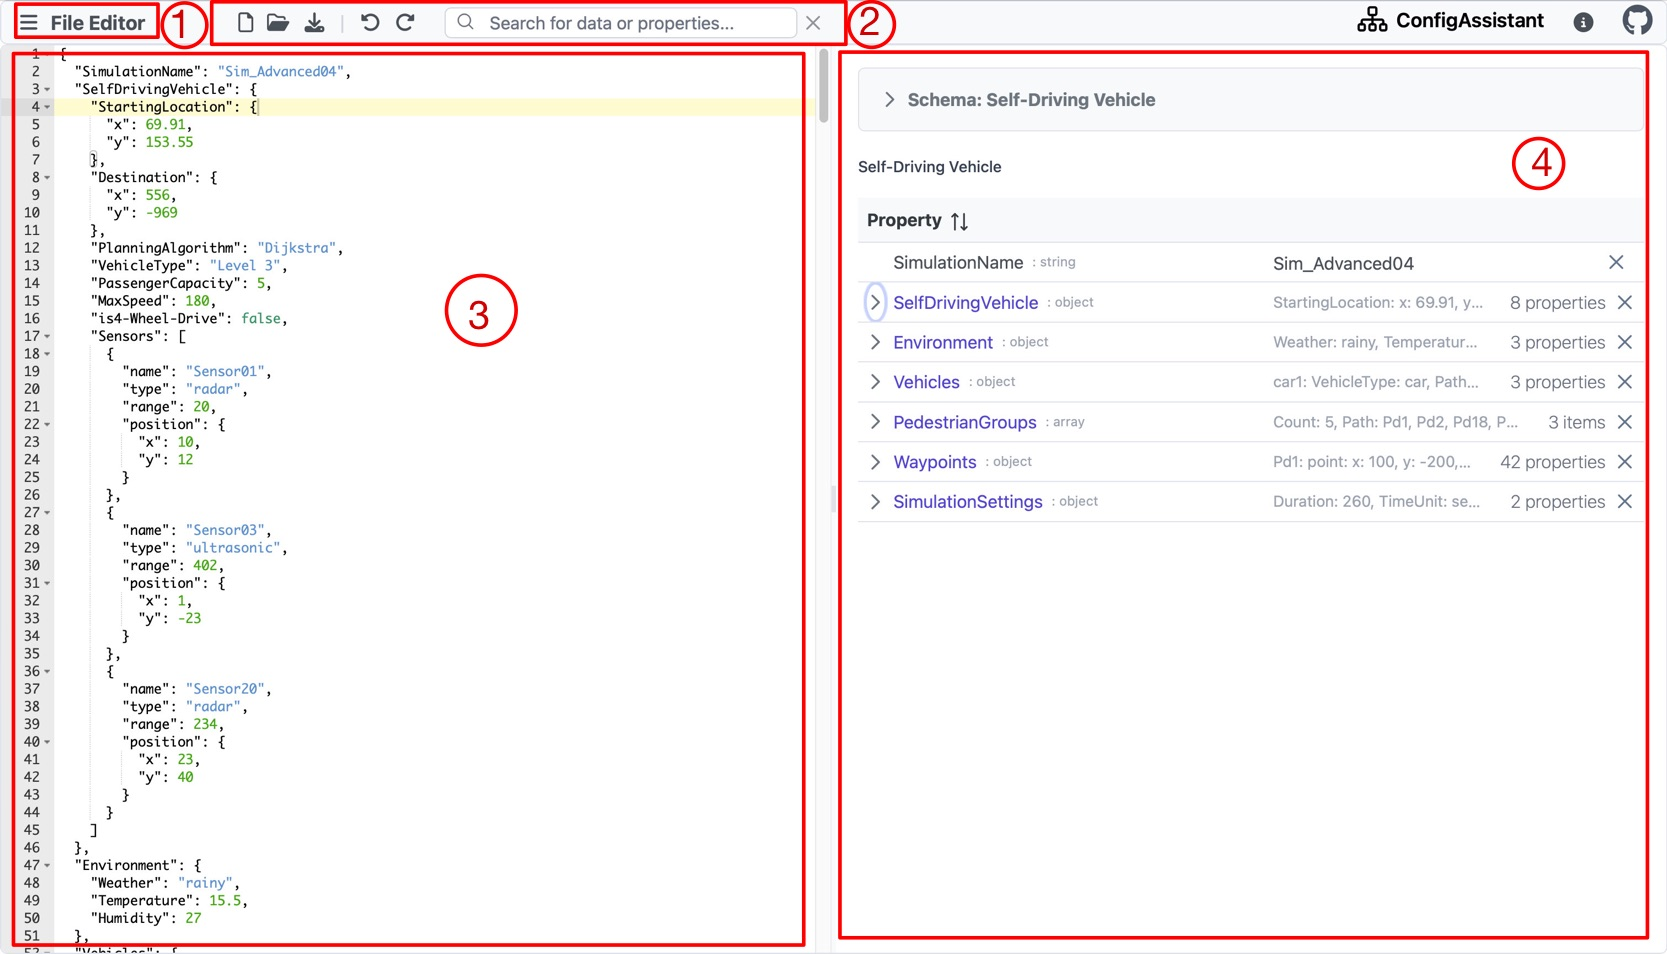
\includegraphics[width=\textwidth]{figures/fileeditor}
    \caption{FileEditor}
    \label{fig:fileeditor}
\end{figure*}

\begin{figure*}
    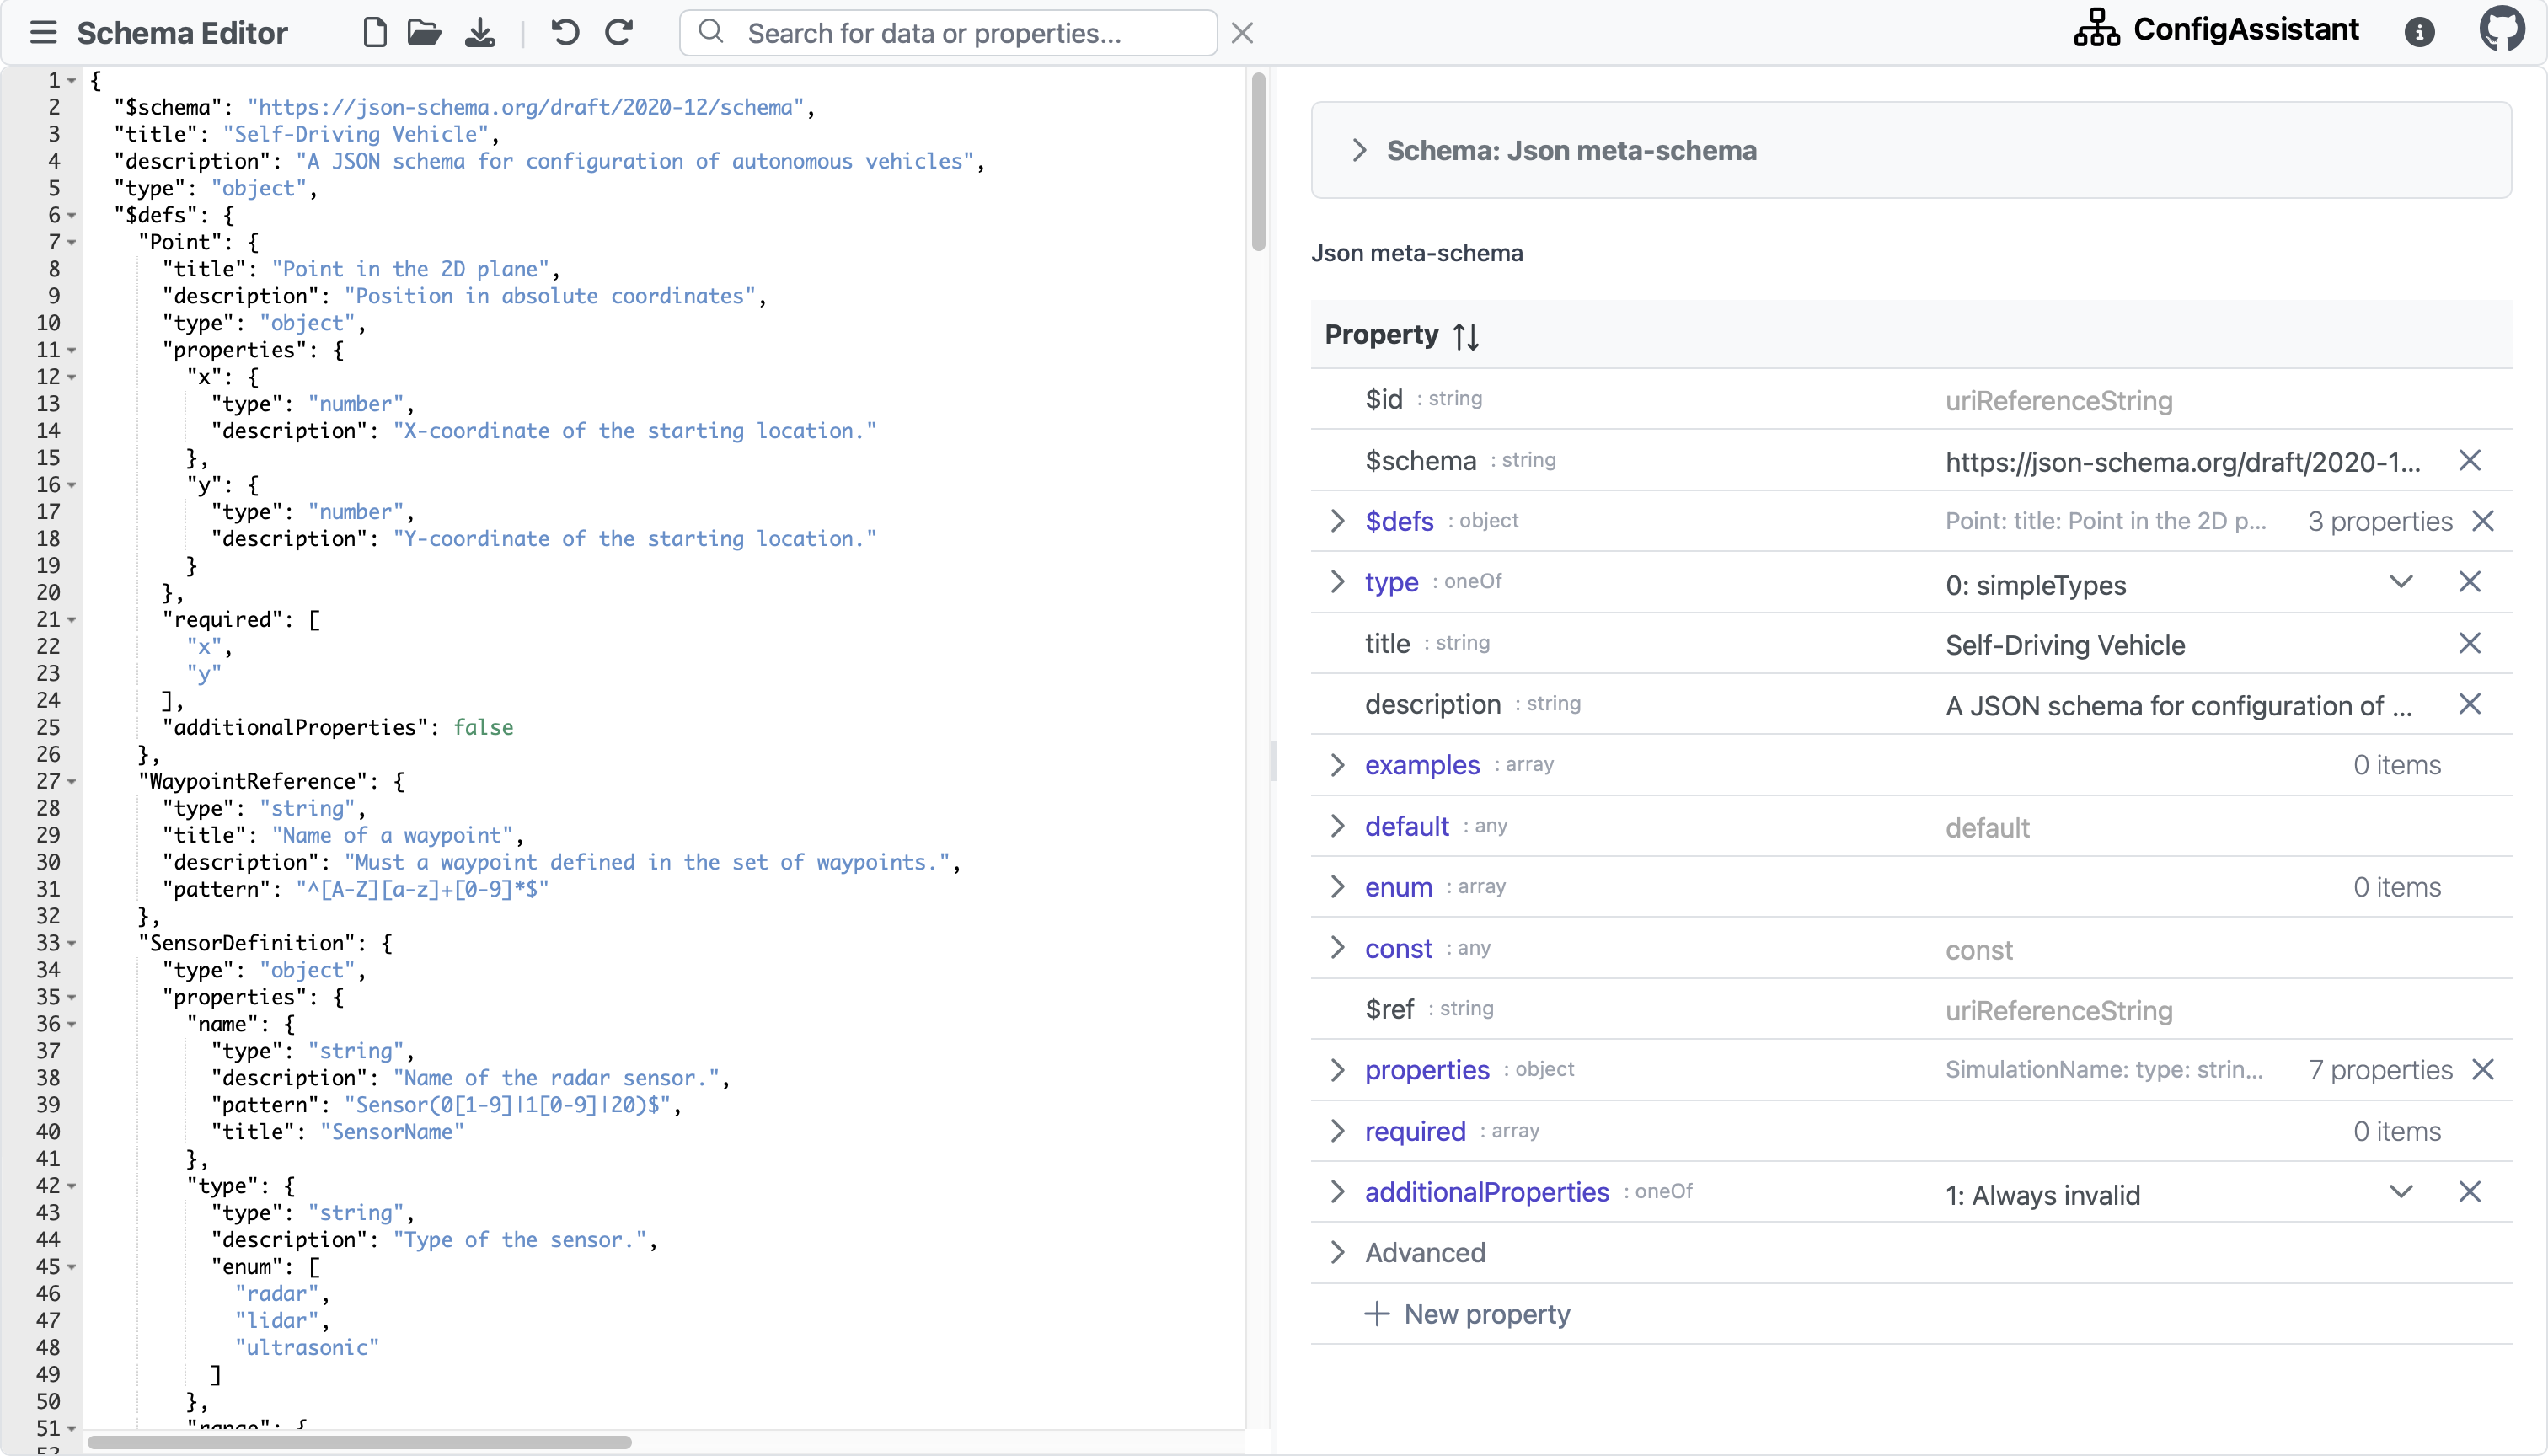
\includegraphics[width=\textwidth]{figures/schemaeditor}
    \caption{SchemaEditor}
    \label{fig:schemaeditor}
\end{figure*}

\begin{figure*}[h]
    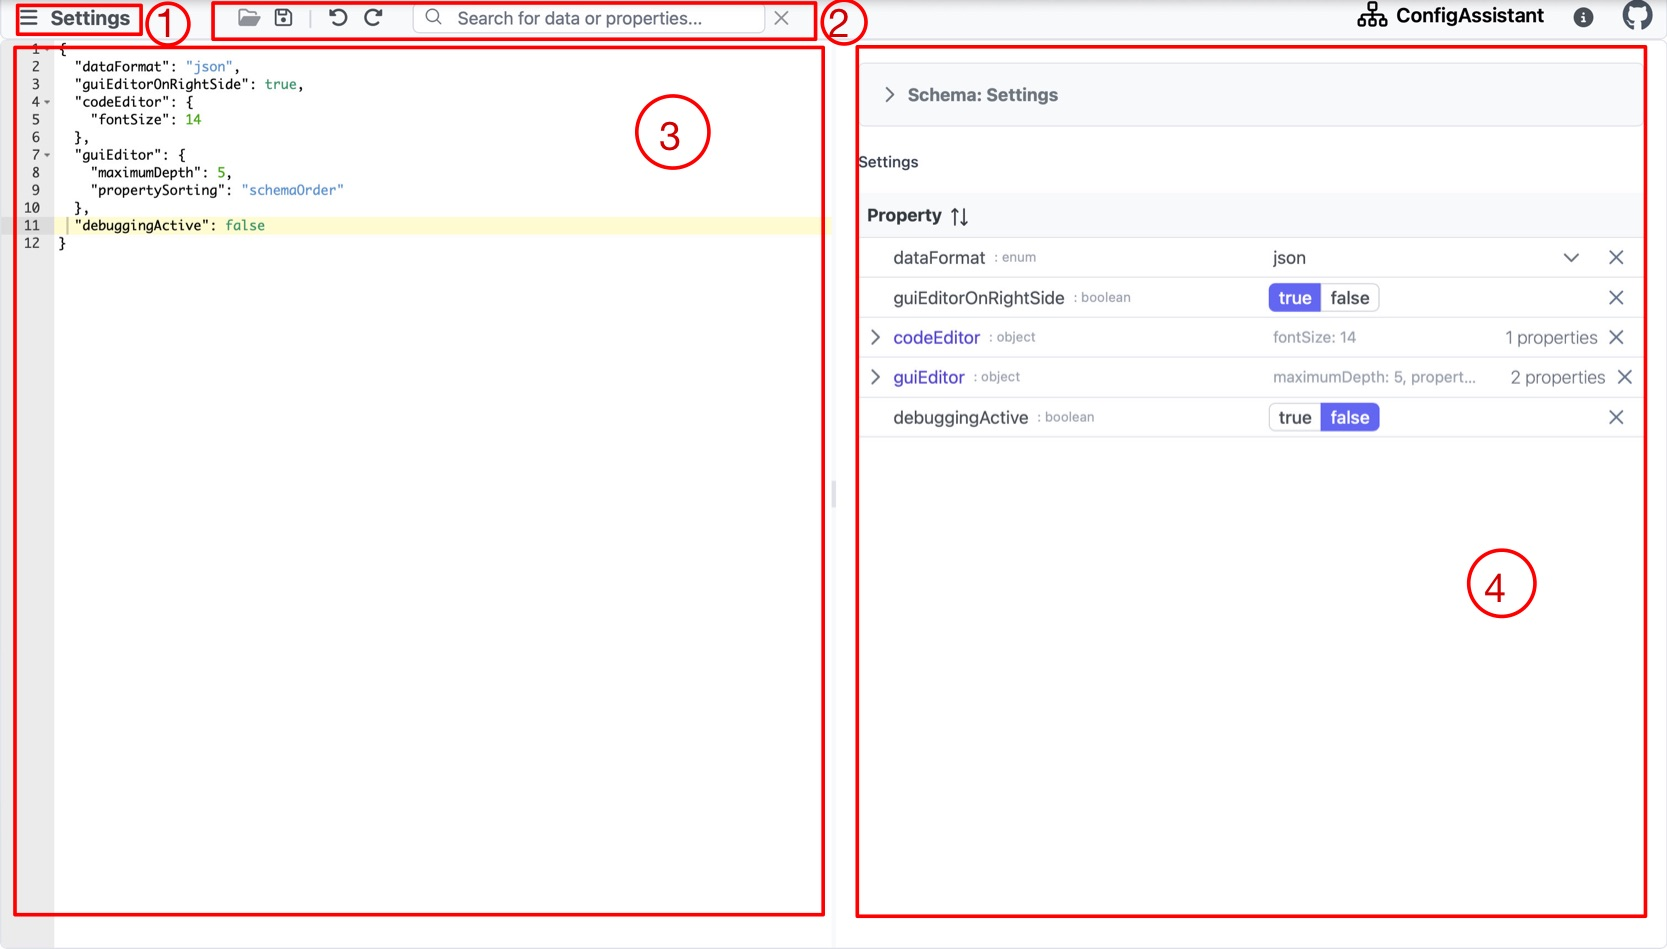
\includegraphics[width=\textwidth]{figures/settings}
    \caption{Settings}
    \label{fig:settings}
\end{figure*}

\subsubsection{Toolbar functionalities}

The toolbar provides basic functionalities for all three views:
\begin{itemize}
    \item {New File: Create a new (schema) file.
    In the file editor, this option also includes two sub-items:
    \begin{itemize}
        \item Generate Data: Generate random configuration data based on the selected schema from the Schema Editor.
        \item New Empty File: Start with a blank file, discarding any current changes.
    \end{itemize}

    \item Open File: Open an existing file.
    For the File Editor, this opens a dialog to open a file from the local file system.
    For the Schema Editor, this comes with four sub-options:
    \begin{itemize}
        \item JSON Schema Store: Choose a schema from the JSON Schema Store, which provides a list of available schemas.

        \item From Our Examples: Access four example schemas provided within the tool.

        \item From File: Select a schema from local file system.

        \item From URL: Provide the URL of a specific schema, and the tool will retrieve and open it.

    \end{itemize}
    \item Undo/Redo: Undo or redo the latest operations in the editor.
    \item Download: Download the current editor content with an appropriate file name.
    \item Search: Text field where the user can enter a search term to find and navigate to specific sections within the current file.
\end{itemize}


\subsubsection{Settings}

In the Settings view (figure~\ref{fig:settings}), the user can adjust various parameters (tab~\ref{tab:settings})of \toolname{}:
\begin{table*}
    \centering
    \caption{Setting Parameters\label{tab:settings}}
    \begin{tabular}{@{}p{0.3\linewidth}p{0.6\linewidth}@{}}
        \toprule
        \textbf{Parameter} & \textbf{\ Description} \\
        \midrule
        Data Format & The data format used by the code editor. Currently YAML and JSON are supported. \\
        Code Editor Font Size & Size of the font in the code editor. \\
        Gui Editor On Right Side & By default, the GUI panel is located on the right side and the code panel on the left side. Using this option, their positions can be swapped. \\
        GUI Editor Property Sorting & The order in which the properties in the GUI panel should appear:
        \begin{itemize}
            \item \textit{Schema Order}: Orders elements according to the order in the schema.
            \item \textit{Priority Order}: Orders elements based on their priority (e.g. required properties first, deprecated properties last).
            \item \textit{Data Order }: Orders elements the same way as it is in the data.
        \end{itemize} \\
        GUI Editor Maximum Depth & Determines the maximum level of nesting or hierarchy displayed in the GUI editor. \\
        Debugging Active & For debugging purposes, users can enable or disable the debugging panel as needed.  \\
        \bottomrule
    \end{tabular}
\end{table*}


\subsection{Code Panel}\label{subsec:code-editor}

The code editor is a GUI panel designed for editing the \cfgfiles.
For this project, we use the popular \textit{Ace Editor}\cite{Ace-Editor} library to embed an interactive code editor into our user interface.
% It is a browser based editor that matches and extends the features, usability and performance of existing native editors such as TextMate, Vim or Eclipse.
% It can be easily embedded in any web page or JavaScript application.

\subsubsection{Features}

To make our code editor more user-friendly, we implemented several features, which are described in the following.

\paragraph{Schema Validation}
To provide the user feedback on whether their data is valid according to the provided schema, we perform schema validation.
We make use of the \textit{Ajv JSON schema validator}\cite{ajv-validator} library, which supports the newest JSON schema draft 2020-12.
%Ajv firstly generates a fast validation function from the input schema.
If schema violations are found, the corresponding user data lines in the code editor will be marked with a red error hint, which also describes the violation.


\paragraph{Syntax Highlighting}
Ace Editor supports syntax highlighting for both JSON and YAML, which we use.
The data format can be switched in the \textit{Settings} page.
Note that Ace Editor allows to collapse/expand segments of the text, based on the hierarchical tree structure of the data.

\paragraph{Linkage of text with the data model}
As described in section \ref{subsubsec:design_text_editor_panel}, to map a cursor position in the text editor to a path in the data model we need to implement the function \textit{determinePath(editorContent, cursorPosition)} and to map a path in the data model to a text row in the editor, we need to implement the function \textit{determineRow(editorContent, dataPath)}. For every data format to be supported, those two functions need to be implemented.

For \textit{JSON}, the functions have been implemented using a \textit{Concrete Syntax Tree (CST)}.
The text content is parsed as a CST. Then the tree is is traversed recursively.
Every tree node has a range property, describing the start and end index of the text belonging to the node.
To determine the corresponding path for a cursor position, the cursor position is translated to a character index $targetCharacter$ within the text.
Then the CST is traversed and for all nodes $currentNode$ of type array or object for which $targetCharacter \in currentNode.range$,
the child nodes are checked and the key of the node (or index for array elements) is appended to the result path.
This way, the corresponding path is built up.
To determine the cursor position for a given path, the reverse is done: the CST is traversed until the effective path of the $currentNode$ is the target path. Then $currentNode.range.start$ is returned as result index, which is then translated into a cursor position (row and column).

For \textit{YAML}, this linkage is not yet implemented and will be part of further work.

\paragraph{Editor Operations}
The code editor has more functionalities, such as the possibility to open a file by drag and drop into the editor, as well as customizable font sizes.

\subsection{GUI Panel}\label{subsec:gui-editor}

The GUI editor is a component that allows the user to edit the configuration data in a GUI, which is generated based on the schema of the configuration data.
It is structured in a table-like way, where each row represents a key-value pair of the configuration data.
Arrays elements are represented similarly, where the index of the array element is the key and the value is the array element itself.
Figure~\ref{fig:gui-editor} shows the GUI editor component with an example schema and configuration data.

\begin{figure}[!t]
    \centering
    \includegraphics[width=\columnwidth]{figures/gui-editor} % todo replace with screenshot
    \caption{GUI Editor Component}
    \label{fig:gui-editor}
\end{figure}

To allow this representation of the schema, we do some preprocessing of the schema, which is described in section~\ref{subsec:schema-preprocessing}.

\subsubsection{Features}\label{subsubsec:gui-editor-features}

To assist the user in editing the configuration data, the GUI editor offers a set of features, which are described in the following.

\paragraph{Traversal of the Data Tree}
By default, only the first level of the data tree is shown.
The user can expand the data tree by clicking on the arrow next to the key of an object or array.
This will show the sub-properties of the object or the elements of the array.
We limit the depth of the data tree to a configurable value, to prevent the GUI editor becoming too overwhelming.
However, the user can also click on the property name or array index to \textit{zoom in} to that element.
This will show the sub-properties of that element at the top level, as if that property was the root of the data tree.
The breadcrumb at the top allows the user to see which path the GUI editor currently shows and to navigate back to upper levels of the tree.

% todo add figure to illustrate (for all the different data types and features)

\paragraph{Type specific components}

TODO
% todo write

\paragraph{Remove Data}
The user can delete properties or array elements from the data by clicking on the $\times$ button next to the edit field.
This button is only shown if the property is not required and there exists data.

\paragraph{Schema Information Tooltip}
When the user hovers over the property key or array index, an overlay is displayed, which contains all information from the schema about that property.
We manually implemented a generation of a textual description for each of the JSON schema keywords.
Starting with title and description of the property, the overlay then shows constraints (such as the number must be greater than 0) and in the bottom it also shows schema violations, in case there are any.
This feature helps the user to understand the constraints and the meaning of a property.

\paragraph{Highlighting Schema Validation Errors}
When the configuration data does not comply to the schema, the corresponding elements are underlined in red and highlighted with a red error icon.
This way, the user knows where any errors are.
Additionally, the schema information tooltip lists all schema violations.
% todo add screenshot

\subsection{Schema preprocessing}\label{subsec:schema-preprocessing}

To represent the schema in the GUI editor, we preprocess the schema.
We differentiate between three ways of preprocessing:
A one-time preprocessing step when loading the schema, an internal preprocessing that happens at every layer of the schema tree,
and calculating an effective schema that happens every time the configuration data changes.

\subsubsection{One-time Preprocessing Step}
When the schema is loaded, we perform a one-time preprocessing step that currently only involves migrating the schema to the newest version,
as described in section~\ref{subsec:json-schema-versions}.
The user will be informed about this step and also prompted with a dialog, when the schema file does not define which JSON schema version it uses.
After the migration, the resulting schema is loaded into the tool in the \textit{Schema Editor} page.

% todo maybe describe how bundling might make sense here

\subsubsection{Internal preprocessing}
This preprocessing steps are mainly used to generate the GUI editor and thus are internal steps that will not be visible for the user.
They happen at every layer of the schema tree lazily, only when required.
Laziness of the preprocessing is required as schemas can have circular references, which would, otherwise, lead to infinite loops.
In the following, we describe the preprocessing steps in details.

\paragraph{Resolving references}
JSON schema uses the \texttt{\$ref} keyword to reference other schemas.
This can either be references to schemas in the same file (using the \texttt{\$defs} keyword), references to other local files,
or references to schemas at a URL in the web.
We currently only support references to schemas in the same file.
These are lazily resolved as the first preprocessing step.
Listing~\ref{listing:preprocessing-example} shows an example schema, Listing~\ref{listing:reference-resolving} shows the equivalent example after
this first preprocessing step.

\begin{lstlisting}[language=json,firstnumber=1,caption=
    {Simple JSON schema before reference resolving},captionpos=b]
{
  "title": "NonEmptyString",
  "$ref": "#/$defs/nonEmptyString",
  "$defs": {
    "nonEmptyString": {
      "type": "string",
      "minLength": 1
     }
  }
}
\end{lstlisting}\label{listing:preprocessing-example}

\begin{lstlisting}[language=json,firstnumber=1,caption=
    {Simple JSON schema after reference resolving},captionpos=b]
{
  "allOf": [
   {
     "title": "NonEmptyString"
   },
   {
     "type": "string",
     "minLength": 1
   }
  ],
  "$defs": {
    "nonEmptyString": {
      "type": "string",
      "minLength": 1
     }
  }
}
\end{lstlisting}\label{listing:reference-resolving}

\begin{lstlisting}[language=json, firstnumber=1, caption=
    {Simple JSON schema after allOf resolving}, captionpos=b]
{
  "title": "NonEmptyString"
  "type": "string",
  "minLength": 1,
  "$defs": {
    "nonEmptyString": {
      "type": "string",
      "minLength": 1
     }
  }
}
\end{lstlisting}\label{listing:resolved-allOf}

\paragraph{Resolving allOfs}

The \texttt{allOf} keyword in JSON schema specifies that all of the schemas in the given array must be valid.
To simplify any other operation on the schema, we aim to merge the schemas in the allOf array to one equivalent schema.
As the first step, we do a recursive step by preprocessing all the schemas of the allOf array.
Then, we use the \textit{mergeAllOfs} library % todo citation
for this task.
Listing~\ref{listing:resolved-allOf} shows the previous example schema after this step.
It is important to note that this library only supports a few keywords of JSON schema, most notably the
\texttt{properties} and \texttt{items} keyword.
Hence, the support for allOf and any other keywords for which we use this in the preprocessing is limited.

\paragraph{Converting types to oneOf}
In JSON schema, a property can have multiple supported types, such as shown in listing \ref{listing:multiple_types}.
A semantically equivalent schema can be generated by the use of oneOf, where each sub-schema contains exactly one of the types, as shown in listing \ref{listing:multiple_types_converted}.
If a schema defines more than one type, we convert the types to oneOf. This way, we reduce complexity by having to solve only the problem of oneOf.
For schemas that already contain oneOf, every type is multiplied with every existing oneOf sub-schema.
For 2 types and 3 oneOf sub-schemas, this will result in a new oneOf with 6 options.
An exception is when a type can not be merged with an oneOf sub-schema (e.g. the type is "boolean" and the oneOf sub-schema has type "string").
In that case, the incompatible pair is dismissed.

\begin{lstlisting}[language=json, firstnumber=1, caption=
    {Simple JSON schema with two possible types}, captionpos=b]
{
  "type": ["object", "boolean"]
}
\end{lstlisting}\label{listing:multiple_types}

\begin{lstlisting}[language=json, firstnumber=1, caption=
    {Simple JSON schema after conversion of types to oneOf}, captionpos=b]
{
  "oneOf": [
    {
      "type": "object"
    },
    {
      "type": "boolean"
    },
  ]
}
\end{lstlisting}\label{listing:multiple_types_converted}


\paragraph{Removing incompatible oneOfs and anyOfs}
It can happen that a schema has oneOf or anyOf options which are not compatible with the schema of the property (e.g.\ sub-schemas that can never be fulfilled in combination with the property schema).
Listing~\ref{listing:incompatible_one_ofs} provides an example of a schema with an incompatible oneOf option.
An example where this occurs is in our adjusted JSON schema meta schema, if we assign the root property the jsonSchema sub-schema, which allows objects and booleans, but then additionally restrict the root to be an object.
For every oneOf and anyOf sub-schema, we check whether it can be merged with the schema of the property.
The options which are not compatible (can not be merged) are removed (see listing~\ref{listing:incompatible_one_ofs_removed}).

\begin{lstlisting}[language=json, firstnumber=1, caption=
    {Simple JSON schema with incompatible oneOf option}, captionpos=b]
{
  "type": "object",
  "oneOf": [
    {
      "type": "object"
    },
    {
      "type": "boolean"
    },
  ]
}
\end{lstlisting}\label{listing:incompatible_one_ofs}


\begin{lstlisting}[language=json, firstnumber=1, caption=
    {Simple JSON schema with incompatible oneOf option removed}, captionpos=b]
{
  "type": "object",
  "oneOf": [
    {
      "type": "object"
    }
  ]
}
\end{lstlisting}\label{listing:incompatible_one_ofs_removed}


\paragraph{Merging singular oneOfs and anyOfs}
Because of the previous pre-processing step, it can happen that for some oneOfs or anyOfs there remains only one compatible sub-schema left (see listing \ref{listing:incompatible_one_ofs_removed}).
If this is the case, the use oneOf/anyOf is redundant, as that singular sub-schema must be chosen implicitly.
Therefore, if there exists only one singular choice for oneOf/anyOf, we merge its sub-schema into the property schema and remove the use of oneOf/anyOf (see listing \ref{listing:singular_one_of_merged}).

\begin{lstlisting}[language=json, firstnumber=1, caption=
    {Simple JSON schema with singular oneOf merged into property schema}, captionpos=b]
{
  "type": "object"
}
\end{lstlisting}\label{listing:singular_one_of_merged}


\paragraph{Attempting to merge oneOfs into anyOfs}
Schemas can use both anyOf and oneOf at the same time.
Especially after converting all types (when there is more than one type) to oneOf, it happens that a schema has oneOf options (typically for types) and simultaneously anyOf options.
The user will then have to select both an oneOf sub-schema, as well as an anyOf sub-schema in the GUI.
We observed a special scenario in the JSON meta schema, where the oneOf selection was always implicitly given by the anyOf selection.
For every single anyOf sub-schema, only one oneOf sub-schema was compatible.
In that scenario, we can merge the oneOfs into the anyOfs: for every anyOf sub-schema, we merge the one compatible oneOf sub-schema into it.
This is precisely what this pre-processing step does: if possible, the oneOf sub-schemas are merged into the anyOf sub-schemas and the oneOf property is removed from the schema.


\paragraph{Preprocessing oneOfs and anyOfs}
For all remaining oneOf and anyOf sub-schemas, the internal pre-processing steps are executed.


\paragraph{Title inducing}

The \texttt{title} keyword is used to give a schema a short description.
This is not necessarily the same as the property name of properties of an object.
As we use the title in various cases to display for the user, we inject the property name in cases where no explicit title is given.

\begin{lstlisting}[language=json, firstnumber=1, caption=
    {Simple JSON schema with one property without a title}, captionpos=b]
{
  "type": "object",
  "properties": {
    "name": {
      "type": "string"
    }
  }
}
\end{lstlisting}\label{listing:no-title}

\begin{lstlisting}[language=json, firstnumber=1, caption=
    {The property names was used for the title field}, captionpos=b]
{
  "type": "object",
  "properties": {
    "name": {
      "title": "name",
      "type": "string"
    }
  }
}
\end{lstlisting}\label{listing:with-title}

\paragraph{Processing enum and const}
The enum keyword is used to restrict the values of a field to a fixed set of valid values.
The const keyword, similarly, restricts the property value to a single allowed value.
Thus, setting the const value is equivalent to settings the enum value with an array that contains this single value.

We convert any usage of const to enums with a single element, which allows us to ignore the const keyword in other operations.

\subsubsection{Calculating an effective schema}

This third preprocessing step is calculated the most often, namely every time the data changes.
However, for most schemas this preprocessing step is trivial.
The JSON schema keywords \texttt{if}, \texttt{then}, and \texttt{else} provide a way to include conditions in the JSON schema.
If the schema in the \texttt{if} field is valid, then also the schema in the \texttt{then} field must be valid, otherwise the
schema in the \texttt{else} field must be valid.

This makes the schema data dependent.
To show the correct properties, we evaluate the data and dependent on validity or not, we either use the \texttt{then} or the \texttt{else} schema.

We similarly handle the \texttt{dependentRequired} and the \texttt{dependentSchemas} keywords.
For schemas without any of those keywords, this step is trivial as the schema is not modified in any way.

%todo examples

\subsection{Schema editor}\label{subsec:schema-editor}

The schema editor page has the same structure as the File editor page, as discussed in previous sections.
The only difference is that the schema used for generating the GUI panel is not the schema file provided by the user but the Json schema meta schema,
i.e., the schema that defines the structure of valid JSON schema files.
However, applying our generic approach on the official Json schema meta schema (TODO citation) does not result in a user-friendly editor for
creating and modifying schema files.
In this section we discuss the reasons for that and how we developed a new meta schema that circumvents the problems of the official meta schema.

\subsubsection{Missing descriptions}
With the \texttt{description} keyword, schema authors can give descriptions to any elements of their schema.
This can help the user of a schema in many ways, for example, the author can specify the unit of a numeric field or give other additional information.
The JSON schema meta schema does not provide any descriptions.
Users, especially those without prior knowledge in JSON schema, might not understand the meaning of the fields of JSON schema.
Thus, we insert descriptions from the JSON schema specification (TODO citation) into our modified meta-schema.

\subsubsection{External references}
\toolname does not support references to external schemas yet, i.e., references inside the schema to a schema at a specific URL\@.
Also, \toolname does not support the \texttt{\$vocabulary} keyword yet.
Both features are used in the JSON schema meta schema, as it is distributed over multiple schema files.
To circumvent that problem, we put all schemas in one schema file into the \texttt{\$defs} object and replace the external references with local references.

\subsubsection{Use of dynamic anchors and references}
The JSON schema meta schema uses dynamic references and dynamic anchors.
The difference of those keywords in comparison to the \texttt{\$ref} keyword is that they provide a way to dynamically extend the JSON meta schema
at runtime.
For example, one could combine the JSON schema meta schema with an extension that defines how fields should be serialized in XML\@.
We do not support dynamic references and anchors yet.
We replaced all of them by ``non-dynamic'' references using the \texttt{\$ref} keyword.

\subsubsection{Allowing each field in each context}
The JSON schema meta schema allows each field in each context.
For example, if the \texttt{type} keyword is used and set to \texttt{string}, then the \texttt{properties} keyword is allowed,
even though it does not make sense in that context.
According to the specification, any validator should ignore the fields that do not make sense in the current context.
Consequently, the user does not need to see those fields, but instead, the user gets overwhelmed by the amount of fields
and does not know which fields are relevant for the current context.
This is also a feedback we got from our user study.

\begin{lstlisting}[language=json, firstnumber=1, caption=
    {If condition for array properties. The \texttt{hasTypeArray} is valid if the current property is of type array. The \texttt{arrayProperty} schema defines the properties of an array.}, captionpos=b]
{
  "if": {
    "$ref": "#/$defs/hasTypeArray"
  },
  "then": {
    "$ref": "#/$defs/arrayProperty"
  }
}
\end{lstlisting}\label{lst:if-then-else}

Thus, we added \texttt{if} conditions to each field to only show them when they make sense in the current context.
Listing~\ref{lst:if-then-else} shows an example of such an \texttt{if} condition.
The relevant properties for arrays are only shown when the current property is of type array.

To even more reduce the amount of fields shown to the user, we also introduced a custom keyword just for our own meta schema.
The keyword \texttt{advanced} is a boolean field that is set to \texttt{false} by default.
It is wrapped in an \texttt{metaConfigurator} object, which is ignored by any validator as it is not part of the JSON schema specification.
We use this wrapper to prevent any other schema extensions from colliding with our keyword.
When set to \texttt{true}, the field not shown by default, but only when the user expands the advanced section.
We put all fields that are not required for the basic usage of the schema into the advanced section.
For this, we oriented ourselves on the work of Baazizi et al.~\cite{baazizi2021empirical}, which analyzed the usage of JSON schema keywords in 82,000 JSON schemas.

% TODO screenshots


% paul
% todo consider putting somewhere else
\subsection{JSON schema versions}\label{subsec:json-schema-versions}

JSON schema has had 10 different drafts over the years, the newest being draft 2020--12~\cite{jsonschemaJSONSchema}.
In real-world we cannot expect all schemas to have the newest version.
Baazizi et al.~\cite{baazizi2021empirical} investigated over 82.000 open-source schemas in 2021, where they found that most of them are using draft 4, which was released in 2013.
As the different drafts are not necessarily compatible with each other, tools supporting one draft become outdated when a new draft releases.
However, Viotto et al.~\cite{Viotti_Lagoni_2023} provide a library for migration schemas from older versions to the newest draft without loss of information.
Thus, by using this library, our tool only needs to support the newest draft directly.
If a user uses a schema from an older draft, we first migrate it to the newest draft internally.
